\documentclass[10pt,a4paper]{article}
\usepackage[margin=2.5cm]{geometry}
\usepackage[T1]{fontenc}
\usepackage{lmodern}
\usepackage{microtype}
\usepackage{amsmath,amssymb}
\usepackage{graphicx}
\usepackage{booktabs}
\usepackage{caption}
\usepackage[hidelinks]{hyperref}
\usepackage[section]{placeins}
\captionsetup{font=small,labelfont=bf}
\graphicspath{{figures/}}

\title{When Do Depth Priors Help Sparse-View 3D Gaussian Splatting?\\[3pt]
\large A Controlled Study of Appearance, Geometry, and Prior Corruption}
\author{Ameer Alayan \qquad Moneer Ghanem\\[6pt]
\small The Hebrew University of Jerusalem\\
\small Deep Learning for 3D Computer Vision --- Final Project}
\date{}

\begin{document}
\maketitle

\begin{abstract}
Monocular depth can regularize sparse-view 3D Gaussian Splatting (3DGS), but an
inaccurate prior may also constrain reconstruction toward the wrong geometry. We
study this interaction through 257 completed runs spanning initialization, view
count, depth-loss family and weight, controlled corruption, and Depth Anything V2.
On NeRF-Synthetic, clean dense-reference initialization substantially improves both
held-out PSNR and reference-depth agreement; exact depth rendered from the original
Blender scenes confirms the dense reference to within 0.4\% on the scenes used for
corruption. Corruption can reverse this advantage: in a three-view noise experiment,
joint improvement at 3.9\% prior AbsRel becomes joint degradation at 7.9\%. This is
a transition between sampled settings, not a universal error threshold. Error
structure also matters: coherent scale errors produce much greater reference-depth
error than larger pixelwise noise. Selected experiments exhibit opposing changes in
PSNR and geometry, while many corrupted conditions degrade both. Depth Anything V2
yields useful synthetic results with reference-assisted calibration but poor results
at the tested sparse-SfM calibration operating point. On two real DTU scans, its
depth initialization reduces structured-light Chamfer error by 45\% relative to
random initialization at three views. Adding reference-depth supervision further
improves DTU geometry, although PSNR, SSIM, and LPIPS do not always agree on
appearance. The practical lesson is to assess calibration, intervention path, and
geometry alongside multiple image-quality metrics before trusting a depth prior.
\end{abstract}

\section{Introduction}

3D Gaussian Splatting (3DGS) represents a scene with explicit, differentiable
Gaussian primitives and can synthesize high-quality novel views
efficiently~\cite{kerbl2023}. With only a few training views, however, image
reconstruction alone leaves substantial geometric ambiguity. A set of primitives may
fit the observed images while placing surfaces incorrectly or producing unstable
depth in unseen views. Monocular depth offers a dense additional constraint, either
by supplying initial 3D points or by supervising rendered depth during optimization.

The usefulness of this constraint depends on what the prior gets wrong. Local noise,
a coherent scale error, and image-dependent scale or shift can have different effects
even at similar average depth error. Moreover, an image-quality gain does not
establish geometric improvement. This distinction matters when a reconstruction will
be used for measurement or downstream 3D processing rather than only novel-view
rendering.

We investigate three questions. First, how do initialization and the number of views
affect the value of clean depth? Second, how do the intervention path, depth loss,
and corruption structure change the result? Third, do controlled synthetic
observations extend to a real monocular estimator and to independently measured
real-scene geometry? We address these questions with a staged experiment over 257
completed runs, using NeRF-Synthetic for controlled reference-depth perturbations and
DTU structured-light scans for external geometric evaluation.

Our contribution is a controlled diagnostic study rather than a new rendering method.
It separates initialization from continued depth supervision, compares three depth
losses, and relates prior error to both appearance and geometry. The results show
strong clean-prior benefits, substantial joint failures under corrupted priors, and
concrete cases of PSNR--geometry divergence. They also show why a single appearance
score or a universal prior-error cutoff is an inadequate basis for choosing depth
supervision.

\section{Related Work}

\paragraph{Gaussian splatting and initialization.} Kerbl et al.~\cite{kerbl2023}
introduced anisotropic 3D Gaussians, differentiable splatting, and adaptive density
control for real-time radiance-field rendering. The initial point distribution is
consequential because optimization and densification start from it. Foroutan et
al.~\cite{foroutan2024} study alternatives to SfM initialization, including random
initialization and structure distilled from NeRF, and find that carefully designed
random initialization can approach SfM. This motivates treating initialization as an
experimental variable rather than a fixed preprocessing choice. Here we examine it under sparse supervision and
explicitly measure depth agreement in addition to image quality.

\paragraph{Depth-regularized sparse-view reconstruction.} DNGaussian~\cite{li2024}
uses hard and soft depth regularization with global--local normalization. It
explicitly discusses conflicts between coarse monocular depth and detailed
appearance. Our study complements such methods by holding the reconstruction framework fixed while varying the quality and
entry point of depth information. We do not claim to introduce the
appearance--geometry conflict; we characterize it with controlled corruption and
paired measurements.

\paragraph{Monocular depth and geometric evaluation.} Depth Anything
V2~\cite{yang2024} provides a strong pretrained relative-depth estimator, but its
relative predictions require calibration before use as camera-space depth. We use it
as one empirical operating point alongside synthetic perturbations.
NeRF-Synthetic~\cite{mildenhall2020} supplies calibrated rendered scenes for the
controlled study. DTU~\cite{jensen2014} provides calibrated real images and
structured-light reference geometry, enabling a complementary test beyond agreement
with a learned dense reconstruction.

\section{Method}

Let $\{I_i, K_i, T_i\}_{i=1}^{V}$ be the training RGB images, camera intrinsics, and
camera-to-world transforms. Camera poses are held fixed. A depth prior $P_i$ is
associated with each training image when depth is used. We distinguish the prior from
the reconstruction's rendered depth $\widehat{D}_i$ and from the evaluation reference
$D_i^{\mathrm{ref}}$.

\paragraph{Representation and rendering.} The scene is a set of Gaussians
$\mathcal{G}=\{\mu_j,\Sigma_j,o_j,c_j\}_{j=1}^{N}$, with center
$\mu_j\in\mathbb{R}^3$, positive-definite covariance $\Sigma_j$, opacity $o_j$, and
color coefficients $c_j$. Covariance is parameterized by rotation and positive
scales. Projection produces a 2D Gaussian footprint whose opacity contribution at
pixel $u$ is $\alpha_j(u)$. For primitives sorted front to back, define
\begin{equation}
T_j(u)=\prod_{k<j}\bigl(1-\alpha_k(u)\bigr),\qquad w_j(u)=T_j(u)\,\alpha_j(u).
\end{equation}
The rendered RGB and expected depth are
\begin{equation}
\widehat{I}(u)=\sum_j w_j(u)\,c_j+\Bigl(1-\sum_j w_j(u)\Bigr)c_{\mathrm{bg}},\qquad
\widehat{D}(u)=\frac{\sum_j w_j(u)\,z_j}{\sum_j w_j(u)+\epsilon},
\end{equation}
where $z_j$ is camera-space depth and $\epsilon$ stabilizes division. Expected depth
is an opacity-weighted rendering statistic; it is not itself a mesh or a guarantee of
surface accuracy. We optimize Gaussian parameters using differentiable rasterization
and adaptive densification and pruning.

\subsection{Depth-prior intervention paths}

\paragraph{Initialization.} Random initialization samples points within the
configured scene extent. SfM initialization uses known-pose triangulation: SIFT
features are matched with a ratio test, checked against the known epipolar geometry,
and triangulated with DLT. This isolates point initialization without conflating it
with camera-pose estimation. Depth initialization backprojects valid training pixels.
Writing $T_i=(R_i,t_i)$ and $\tilde{u}=(u_x,u_y,1)^\top$,
\begin{equation}
X_i(u)=R_i\bigl(P_i(u)\,K_i^{-1}\tilde{u}\bigr)+t_i.
\end{equation}
The resulting colored points seed Gaussian centers. Backprojection requires positive
depth in the camera coordinate system; affine-ambiguous relative predictions cannot
be substituted directly as metric depth.

\paragraph{Calibrating Depth Anything V2.} The model predicts relative inverse depth
$d_i(u)$. We calibrate it per image with an affine map in inverse-depth space and
then invert, $P_i(u)=1/\bigl(s_i\,d_i(u)+t_i\bigr)$. The reference-assisted (oracle)
condition fits $(s_i,t_i)$ by least squares to $1/D_i^{\mathrm{ref}}$ over valid
pixels. The SfM-assisted condition fits it to $1/z$ at the triangulated points that
view $i$ helped triangulate, widened to all triangulated points projecting into the
image when fewer than five are available. With three or more points the fit is least
squares followed by one outlier-rejection pass (residuals beyond
$3\times1.4826$ median absolute deviations); with two points it is solved exactly;
with a single point, or when the fit yields a non-positive scale, only the scale is
fitted ($t_i=0$). The calibrated prior is restricted to the foreground mask where one
exists.

We evaluate three intervention paths (Table~\ref{tab:paths}). Initialization only
tests whether the starting geometry remains helpful after RGB optimization. Loss only
asks whether depth can guide a reconstruction initialized without dense depth.
Initialization plus loss tests the combined effect. A corrupted prior can therefore
affect the reconstruction even at $\lambda=0$ if it supplied the initial point cloud.

\begin{table}[!htbp]\centering\small
\caption{Depth intervention paths. The loss-only path uses random or SfM
initialization; each comparison specifies its baseline.}
\label{tab:paths}
\begin{tabular}{lll}
\toprule
Path & Initial Gaussian centers & Depth loss during training\\
\midrule
Initialization only & Backprojected prior & None ($\lambda=0$)\\
Loss only & Random or SfM points & $\lambda>0$\\
Initialization + loss & Backprojected prior & $\lambda>0$\\
\bottomrule
\end{tabular}
\end{table}

\subsection{Training objective and depth losses}

The training objective averages image and depth losses over sampled training views:
\begin{equation}
\mathcal{L}=\mathcal{L}_{\mathrm{RGB}}+\lambda\,\mathcal{L}_{\mathrm{depth}},\qquad
\mathcal{L}_{\mathrm{RGB}}=0.8\,\|\widehat{I}-I\|_1+0.2\bigl(1-\mathrm{SSIM}(\widehat{I},I)\bigr),
\end{equation}
where the $L_1$ term is averaged over pixels and color channels. Depth terms are
computed over valid prior pixels $\Omega$, with $n=|\Omega|$. We compare the following
three losses.

\paragraph{Scale-and-shift alignment loss (SSI).} The implementation first fits a
least-squares affine transformation of rendered depth to the target, then evaluates a
mean absolute residual:
\begin{align}
(s^*,t^*)&=\arg\min_{s,t}\sum_{u\in\Omega}\bigl(s\,\widehat{D}(u)+t-P(u)\bigr)^2,\\
\mathcal{L}_{\mathrm{SSI}}&=\frac{1}{n}\sum_{u\in\Omega}\bigl|s^*\widehat{D}(u)+t^*-P(u)\bigr|.
\end{align}
For nondegenerate depth variation, the least-squares solution is
$s^*=\sum_u(\widehat{D}(u)-\overline{\widehat{D}})(P(u)-\overline{P})/\sum_u(\widehat{D}(u)-\overline{\widehat{D}})^2$
and $t^*=\overline{P}-s^*\overline{\widehat{D}}$, with numerical stabilization in
code. Importantly, fitting uses squared residuals while the final penalty is $L_1$.

\paragraph{Pearson loss.} With $x_u=\widehat{D}(u)-\overline{\widehat{D}}$ and
$y_u=P(u)-\overline{P}$,
\begin{equation}
\mathcal{L}_{\mathrm{Pearson}}=1-\frac{\sum_u x_u y_u}{\sqrt{\sum_u x_u^2}\sqrt{\sum_u y_u^2}+\epsilon}.
\end{equation}
This encourages correlated spatial variation without imposing an absolute scale or
offset. Positive affine changes of the target leave correlation unchanged in the
nondegenerate, unstabilized case.

\paragraph{Absolute depth loss.} For a prior calibrated into the reconstruction's
depth coordinates,
\begin{equation}
\mathcal{L}_{\mathrm{abs}}=\frac{1}{n}\sum_{u\in\Omega}\bigl|\widehat{D}(u)-P(u)\bigr|.
\end{equation}
Unlike the aligned losses, this directly penalizes scale and offset disagreement. It
can anchor correct depth, but it can also impose an incorrect metric target.

The losses differ in units and normalization, so equal numerical $\lambda$ values do
not imply equal regularization strength. In particular, the implemented SSI loss
removes an affine mismatch through fitting, but is not invariant in magnitude to
scaling its target. Ideally, for $a>0$ and unchanged valid pixels,
\begin{equation}\label{eq:ssiscale}
\mathcal{L}_{\mathrm{SSI}}(\widehat{D},aP+b)=a\,\mathcal{L}_{\mathrm{SSI}}(\widehat{D},P).
\end{equation}
Thus target scaling can change the effective loss weight even when the affine
mismatch is fitted away.

\subsection{Controlled prior corruption}

We perturb the dense reconstruction reference while keeping the RGB images and camera
poses fixed. The families are
\begin{align}
\text{zero-mean noise:}\quad & P_i(u)=D_i^{\mathrm{ref}}(u)+\eta_i(u),\qquad \mathbb{E}[\eta_i(u)]=0,\\
\text{global affine:}\quad & P_i(u)=a\,D_i^{\mathrm{ref}}(u)+b,\\
\text{per-image affine:}\quad & P_i(u)=a_i\,D_i^{\mathrm{ref}}(u)+b_i.
\end{align}
The noise control varies perturbation intensity; global affine corruption shares
parameters across images, whereas per-image affine corruption allows inconsistent
calibration across views. The highlighted global conditions are pure scale changes,
$b=0$. Noise intensity and affine jitter are nominal experiment controls; we compare
their realized severity through measured prior AbsRel rather than treating those
controls as interchangeable percentages. Corruptions are applied to prior depth, not
to the evaluation reference.

The staged grid avoids redundant configurations. At $\lambda=0$, changing the unused
loss family cannot create a new intervention. Positive global affine changes are
invisible to ideal Pearson correlation in a loss-only path. For SSI, equivalence
additionally requires accounting for the effective weight in Eq.~(\ref{eq:ssiscale}).
Neither argument removes affine-corrupted depth initialization, which changes the
actual backprojected points. Omitted combinations are therefore design exclusions,
not evidence of successful robustness.

\subsection{Evaluation metrics and matched comparisons}

\paragraph{Appearance.} We evaluate held-out RGB images with PSNR, SSIM, and
LPIPS. PSNR measures pixel error,
$\mathrm{PSNR}=-10\log_{10}(\mathrm{MSE})$ for images in $[0,1]$; higher is better.
SSIM measures local structural similarity and is also better when higher. LPIPS
measures learned perceptual distance and is better when lower. We report all three
where numerical results are available and describe PSNR-specific findings as such.

\paragraph{Reference-depth agreement.} The principal synthetic reconstruction metric
is unaligned mean absolute depth error. Prior quality is measured separately:
\begin{equation}
\mathrm{MAE}(\widehat{D},D^{\mathrm{ref}})=\frac{1}{n}\sum_{u\in\Omega}\bigl|\widehat{D}(u)-D^{\mathrm{ref}}(u)\bigr|,\qquad
\mathrm{AbsRel}(P,D^{\mathrm{ref}})=\frac{1}{n}\sum_{u\in\Omega}\frac{|P(u)-D^{\mathrm{ref}}(u)|}{D^{\mathrm{ref}}(u)+\epsilon}.
\end{equation}
MAE is in scene depth units; AbsRel is dimensionless. Prior AbsRel is an input
diagnostic, not the output reconstruction error. The evaluation pipeline also
computes RMSE and thresholded depth ratios. We emphasize unaligned MAE because an
affine fit before evaluation can remove the very error being studied: a depth map with
the correct shape but the wrong global scale could score almost perfectly after
alignment.

\paragraph{Independent DTU geometry.} For reconstructed points $Q$ and
structured-light points $G$, accuracy averages nearest-neighbor distances from $Q$ to
$G$, and completeness averages distances in the reverse direction. The reported DTU
score is their mean,
\begin{equation}
C_{\mathrm{DTU}}=\frac{1}{2}\left[\frac{1}{|Q|}\sum_{q\in Q}\min_{g\in G}\|q-g\|_2+\frac{1}{|G|}\sum_{g\in G}\min_{q\in Q}\|g-q\|_2\right],
\end{equation}
after the evaluation protocol's spatial filtering. Distances are in millimeters,
without a post-hoc scale-and-shift fit. This is a different measurement from
synthetic reference-depth MAE.

\paragraph{Comparisons.} For a geometry error $E$, we use $\Delta E=100(E/E_0-1)$ and
$\Delta\mathrm{PSNR}=\mathrm{PSNR}-\mathrm{PSNR}_0$. Each baseline matches the
dataset, scene, view count, split, and training setup. Intervention comparisons use
random initialization without depth unless stated otherwise; loss ablations hold
initialization fixed and compare $\lambda>0$ against $\lambda=0$. Scene averages use
the same scenes in both arms. Opposing metric directions establish a particular
divergence, not its frequency across an unbalanced experimental grid.

\section{Experimental Setup}

\subsection{NeRF-Synthetic and the dense reconstruction reference}\label{sec:reference}

The main controlled study uses \emph{Lego}, \emph{Chair}, and \emph{Ship}, with 3,
5, or 9 training views. We use a fixed farthest-view selection for these comparisons,
render at $400\times400$ with a white background, train for 7,000 iterations, and
evaluate 25 held-out views. The main study uses spherical-harmonic degree zero,
restricting view-dependent color as an alternative way to explain sparse
observations. The reproduction experiment instead uses degree three and the published
eight-view DietNeRF split.

For each controlled scene, we fit a separate dense 3DGS reconstruction using all 400
images at $800\times800$, with alpha supervision, and render its expected depth as
$D^{\mathrm{ref}}$. Clean-reference interventions are therefore \emph{oracle
conditions}: their depth is derived from substantially more information than the
sparse training views, including views reserved for sparse-model evaluation. They
measure the potential value of strong geometric information, not the performance of a
deployable sparse-view estimator.

Table~\ref{tab:reference} assesses this reference in two ways. Multi-view consistency
and depth-rank agreement with the released depth images are internal checks: a
reconstruction can be internally consistent and still systematically inaccurate. We
therefore also rendered exact depth from the modified Blender scenes the dataset was
created from, which are not part of the release but are available through the NeRF
issue tracker,\footnote{\url{https://github.com/bmild/nerf}, issues 59 and 198; we
used the community copy \texttt{blend\_files\_fixed.zip}.} at the 25 evaluation views
and at the 16--17 views any split uses as input. These renders reproduce the released
geometry: their silhouettes match the released alpha masks at IoU $\geq 0.997$, and
where exact and reference depth disagree by more than 3\%, the released 8-bit depth
images agree with the exact depth on 95--99.9\% of those pixels.

Against exact depth, the reference has 0.22\% AbsRel on Lego and 0.36--0.38\% on
Chair, but 2.3--2.4\% on Ship, where on about a quarter of the pixels it lies a median
5.7\% in front of the water surface (Figure~\ref{fig:reference}); multi-view
consistency had put Ship at 0.17\%, because a surface displaced consistently in every
view is self-consistent. The corruption and Depth Anything V2 experiments use only
Lego and Chair. Recomputing every corrupted prior against exact depth instead of the
reference changes no prior AbsRel by more than 0.25 percentage points; the smallest
noise level moves from 3.94\% to 3.97\%. Section~\ref{sec:refcheck} examines which
geometry comparisons the reference error could affect.

\begin{table}[!htbp]\centering\small
\caption{Dense-reference quality. Left: internal consistency checks, the median
relative reprojection disagreement between neighboring views and rank correlation with
the released depth PNGs. Right: agreement with exact depth rendered from the Blender
scenes; AbsRel is computed as prior error is ($400\times400$, unaligned), on the
evaluation views and on the input views; the within-1\% fraction is at full
resolution; silhouette IoU compares Blender coverage with the released alpha masks.}
\label{tab:reference}
\begin{tabular}{lccccc}
\toprule
& \multicolumn{2}{c}{Internal consistency} & \multicolumn{3}{c}{Against exact Blender depth}\\
\cmidrule(lr){2-3}\cmidrule(lr){4-6}
Scene & Reprojection & Rank corr. & AbsRel (eval / input) & Within 1\% & Silhouette IoU\\
\midrule
Lego  & 0.043\% & 0.987 & 0.22\% / 0.22\% & 94.8\% & 0.9996\\
Chair & 0.049\% & 0.990 & 0.36\% / 0.38\% & 90.8\% & 0.9997\\
Ship  & 0.171\% & 0.961 & 2.33\% / 2.39\% & 48.3\% & 0.9974\\
\bottomrule
\end{tabular}
\end{table}

\begin{figure}[!htbp]\centering
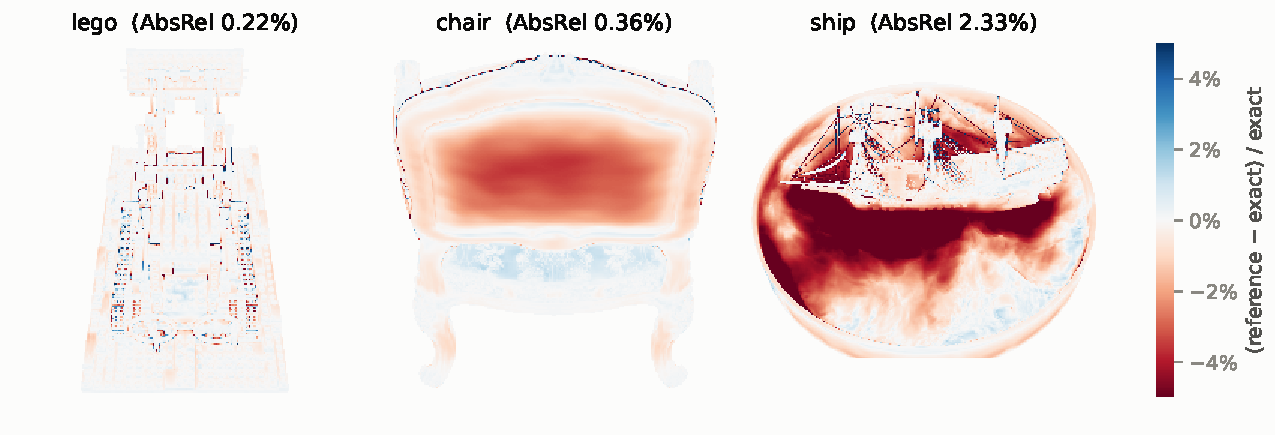
\includegraphics[width=\linewidth]{reference_error.pdf}
\caption{Signed relative error of the dense reference against exact Blender depth on
the first evaluation view (red: reference in front of the true surface; blue: behind).
Lego is exact up to edges; Chair's reference lies 2--4\% in front of the upholstered
back; Ship's lies 5\% and more in front of the water.}
\label{fig:reference}
\end{figure}

\subsection{DTU}

We evaluate scans 1 and 6 from the DTU SampleSet with 3 or 9 training views at
$400\times300$. Cameras use the provided calibration. Structured-light geometry
supplies the independent evaluation target and, in oracle conditions, depth projected
into the training cameras. Evaluation uses 0.2\,mm point downsampling, the
observability mask and ground-plane filtering, and a 20\,mm distance cutoff. We report
the mean of accuracy and completeness. Because the appearance evaluation uses full
images without object masks, these RGB scores should not be compared directly with
masked DTU numbers from other papers.

\subsection{Implementation and reproducibility}

Our implementation uses PyTorch and the installed third-party gsplat 1.5.3
rasterizer~\cite{ye2025}. The authors' code is under \texttt{src/},
\texttt{scripts/}, and \texttt{tests/}; gsplat is a dependency rather than an edited
copy of the rasterizer. Dependencies are specified in \texttt{requirements.txt} and
\texttt{requirements-gpu.txt}. Training uses seeded, automated experiment stages and
supports resuming sweeps. The project repository and executed Colab notebook provide
the setup, training, evaluation, and analysis workflow, including the exact-depth
validation and the scripts that draw the quantitative figures.\footnote{\url{https://github.com/AMEER7525/depth-prior-tax}}

We corrected two integration issues in our code while retaining the rasterizer as an
unmodified installed dependency. We made the packed/unpacked settings of
\texttt{rasterization()} and \texttt{DefaultStrategy} consistent, correcting the
attribution of densification gradients to Gaussians. We also explicitly perform the
vanilla 3DGS opacity reset, correcting an operator-precedence error that prevented the
intended reset condition from firing. These corrections materially improved
reconstruction quality: on Ship, PSNR increased by approximately 1.7\,dB and the
floater fraction decreased from about 45\% to 16\%.

The study contains 257 completed runs across the stages in Table~\ref{tab:stages}.
These runs span different experimental settings; they are not 257 independent
repeated-seed trials. The grid is staged rather than fully Cartesian: broad
initialization and view-count comparisons are followed by loss and corruption studies
and real-scene validation. This design allocates computation to the study's central
questions while retaining matched comparisons within each stage.

\begin{table}[!htbp]\centering\small
\caption{Experimental breadth. Counts describe completed runs in the staged study;
they are not sample sizes for repeated-seed significance tests.}
\label{tab:stages}
\begin{tabular}{lrlr}
\toprule
Stage & Runs & Stage & Runs\\
\midrule
Eight-scene reproduction & 8 & Global affine corruption & 32\\
Initialization $\times$ views & 27 & Per-image affine corruption & 32\\
Initialization/loss combinations & 18 & Synthetic real-model experiment & 20\\
Loss-family/$\lambda$ sweep & 48 & DTU baselines & 8\\
Noise corruption & 40 & DTU reference-depth ablation & 8\\
 & & DTU real-model runs & 16\\
\midrule
 & & Total & 257\\
\bottomrule
\end{tabular}
\end{table}

\section{Results}

\subsection{Reproduction sanity check}

Before interpreting depth interventions, we test the RGB-only implementation against
the 3DGS baseline reported by DNGaussian~\cite{li2024}. Under the eight-view
NeRF-Synthetic protocol, our mean scores are 21.27\,dB PSNR, 0.853 SSIM, and 0.149
LPIPS (Table~\ref{tab:repro}). The corresponding published scores are 22.23, 0.858,
and 0.114. The 0.96\,dB PSNR gap meets our approximate one-decibel sanity criterion,
while the SSIM and LPIPS gaps show that this is not an exact reproduction.
Accordingly, subsequent causal comparisons use our own matched baselines rather than
attributing differences from published systems to depth alone.

\begin{table}[!htbp]\centering\small
\caption{RGB-only reproduction: all eight NeRF-Synthetic scenes, eight-view DietNeRF
split, $400\times400$, 6,000 training iterations, random initialization, SH degree
three. The published comparison is DNGaussian's \emph{3DGS baseline row}, not
DNGaussian itself.}
\label{tab:repro}
\begin{tabular}{lccc}
\toprule
Method & PSNR $\uparrow$ & SSIM $\uparrow$ & LPIPS $\downarrow$\\
\midrule
Our 3DGS implementation & 21.27 & 0.853 & 0.149\\
Published 3DGS baseline~\cite{li2024} & 22.23 & 0.858 & 0.114\\
\bottomrule
\end{tabular}
\end{table}

\subsection{Initialization versus number of views}\label{sec:init}

To isolate initialization, we disable the depth loss and compare reference-depth,
SfM, and random initialization at each view count. Table~\ref{tab:init} and
Figure~\ref{fig:init} show that clean reference depth improves both PSNR and
reference-depth MAE at all three counts. At three views it raises PSNR from 15.00 to
19.43\,dB and reduces MAE from 0.227 to 0.068, a 69.8\% reduction relative to random
initialization. At nine views the corresponding values are 23.65 to 27.14\,dB and
0.084 to 0.026, a 69.5\% reduction.

\begin{table}[!htbp]\centering\small
\caption{Initialization only ($\lambda=0$), averaged over Lego, Chair, and Ship.
Entries are PSNR in dB / unaligned reference-depth MAE in scene units.}
\label{tab:init}
\begin{tabular}{lccc}
\toprule
Initialization & 3 views & 5 views & 9 views\\
\midrule
Clean reference depth & 19.43 / 0.068 & 23.14 / 0.040 & 27.14 / 0.026\\
SfM & 15.51 / 0.254 & 18.97 / 0.129 & 24.99 / 0.058\\
Random & 15.00 / 0.227 & 18.48 / 0.145 & 23.65 / 0.084\\
\bottomrule
\end{tabular}
\end{table}

Additional views improve all three initializations. SfM achieves higher PSNR than
random initialization at 3, 5, and 9 views, but has lower MAE only at 5 and 9 views.
Thus even without a monocular prior, improved image fitting and improved
reference-depth agreement need not coincide. These SfM-versus-random orderings depend
on the scene mix: averaged over Lego and Chair alone, SfM has lower PSNR than random
initialization at 3 and 5 views and lower MAE only at 9 views. The advantage of clean
reference depth, by contrast, holds on both measurements at every view count without
Ship, whose reference is the least accurate (three views: 20.81\,dB / 0.050 against
16.52\,dB / 0.198 for random initialization). The clean-depth results establish an
oracle benefit of informative initial geometry; they do not imply that a real
monocular model supplies equally accurate points.

\begin{figure}[!htbp]\centering
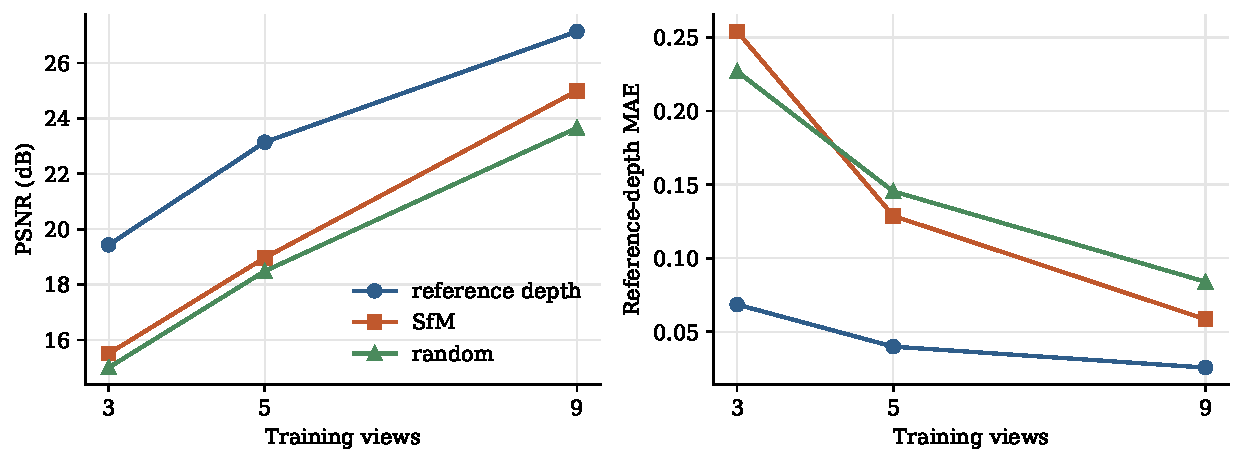
\includegraphics[width=0.92\linewidth]{report_init_views.pdf}
\caption{Initialization and view count. Curves connect the three-scene means in
Table~\ref{tab:init}; they do not depict confidence intervals. Clean-reference
initialization remains beneficial as view coverage increases.}
\label{fig:init}
\end{figure}

\subsection{Depth-loss weight and loss family}

With clean-depth initialization fixed, we sweep SSI, Pearson, and absolute losses over
$\lambda\in\{0.03,0.1,0.3,1\}$ at three and nine views on Lego and Chair.
Figure~\ref{fig:lambda} shows that the effect depends on both loss family and view
count. Pearson deteriorates sharply at the largest weight: the three-view curve ends
near 16.7\,dB PSNR and 0.27 reference-depth MAE. SSI and absolute loss are less
severely affected in this range. At nine views, the SSI curve has lower MAE at the
larger tested weights than at 0.1, whereas the Pearson curve deteriorates strongly at
1. These patterns support tuning the loss within a specified view regime rather than
transferring one weight universally.

\begin{figure}[!htbp]\centering
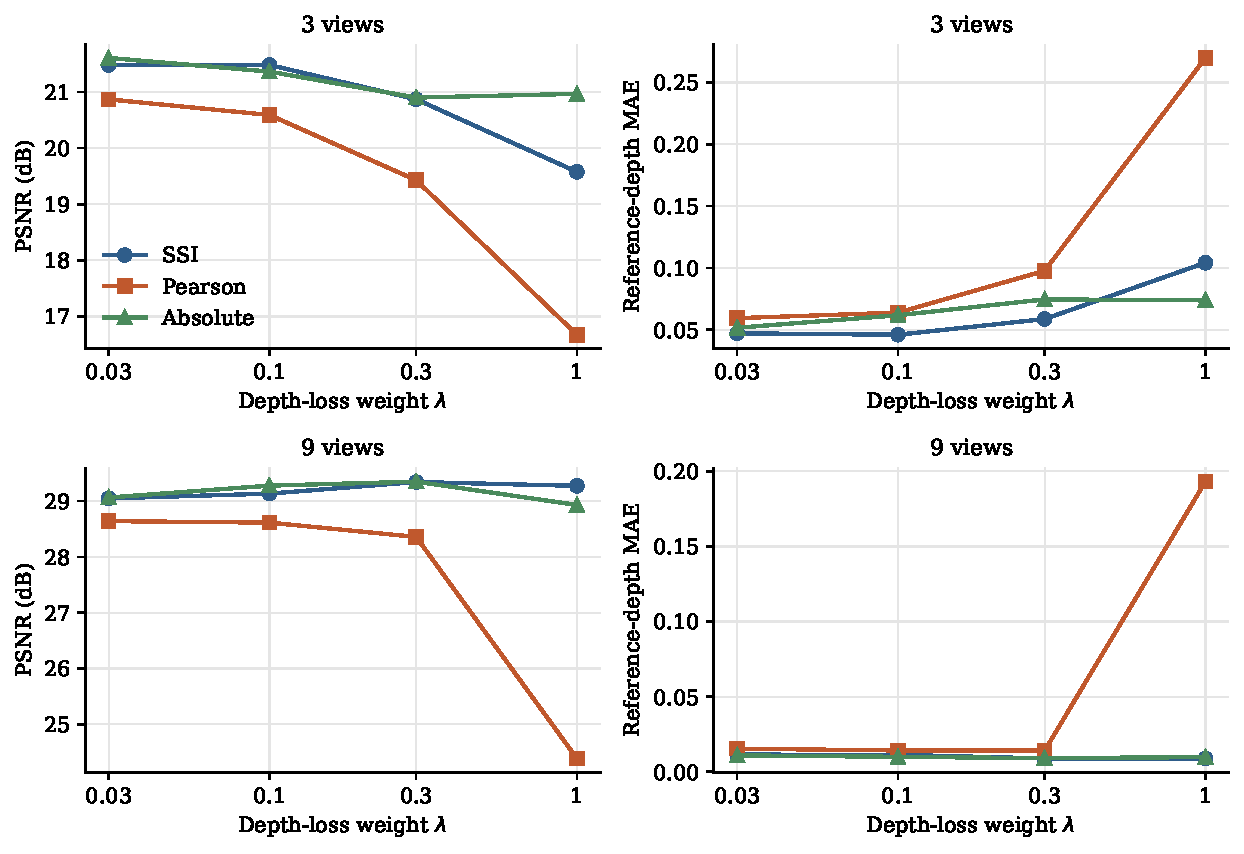
\includegraphics[width=0.92\linewidth]{report_lambda_grid.pdf}
\caption{Clean-prior loss sweep with depth initialization at three and nine views.
Lines summarize the loss-sweep configurations at each tested weight; no repeated-seed
uncertainty is implied. No-loss effects are assessed through the matched scene-level
pairs in Table~\ref{tab:lossablation}.}
\label{fig:lambda}
\end{figure}

Matched single-scene comparisons further show why selecting $\lambda$ by PSNR alone
can be misleading (Table~\ref{tab:lossablation}). On Chair at three views, adding an
absolute loss at $\lambda=0.03$ improves PSNR by 0.95\,dB but raises MAE by 26.0\%.
SSI at the same weight raises PSNR by 0.54\,dB and MAE by 12.1\%. Conversely, on Lego
at nine views, increasing Pearson's weight from 0.1 to 0.3 reduces MAE by 3.6\% while
lowering PSNR by 0.31\,dB. These opposing changes are small in absolute terms, at
most 0.012 in MAE, and lie within the largest shift the reference's own error could
cause (Section~\ref{sec:refcheck}). They show that the two measurements can move
apart under a clean target, but not reliably by how much.

\begin{table}[!htbp]\centering\small
\caption{Selected matched clean-prior loss ablations with depth initialization.
Positive $\Delta$MAE means worse reference-depth agreement. These comparisons are
individual configurations, not significance estimates.}
\label{tab:lossablation}
\begin{tabular}{llcrr}
\toprule
Scene / views & Loss & $\lambda$ change & $\Delta$PSNR (dB) & $\Delta$MAE\\
\midrule
Chair / 3 & Absolute & $0\rightarrow0.03$ & $+0.95$ & $+26.0\%$\\
Chair / 3 & SSI & $0\rightarrow0.03$ & $+0.54$ & $+12.1\%$\\
Lego / 9 & Pearson & $0.1\rightarrow0.3$ & $-0.31$ & $-3.6\%$\\
Lego / 9 & Pearson & $0.3\rightarrow1$ & $-0.21$ & $-2.3\%$\\
\bottomrule
\end{tabular}
\end{table}

We use SSI at $\lambda=0.1$ for the highlighted corruption comparison as a moderate
tested setting. This is an experimental operating choice, not a demonstrated
universal optimum. Since the losses have different scales (Section~3.2), their weight
curves compare implemented objectives, not equally strong constraints.

\subsection{Controlled prior degradation}

To test when the oracle advantage survives imperfect depth, we vary corruption
structure and severity while holding the reconstruction setting fixed.
Table~\ref{tab:corruption} reports the three-view, depth-initialization-plus-SSI
comparison on Lego and Chair. Its matched random-initialization baseline is 16.52\,dB
PSNR and 0.198 MAE; the three-scene mean from Table~\ref{tab:init} is not used for
this comparison.

\paragraph{Noise: a transition between sampled operating points.} At 3.9\% prior
AbsRel, PSNR is 18.32\,dB and MAE is 0.122: a 1.80\,dB gain and a 38.3\% error
reduction. At 7.9\%, PSNR falls to 16.28\,dB and MAE rises to 0.258, reversing both
signs relative to the matched baseline. The 15.7\% condition is worse still, at
14.42\,dB and 0.365 MAE: PSNR decreases by 2.11\,dB and depth error increases by
84.5\%. This locates an empirical transition between the sampled 3.9\% and 7.9\%
conditions. Its location is specific to the scenes, intervention path, loss, and view
setting tested here.

\paragraph{Coherent and image-dependent affine error.} A global scale factor of 0.8
produces 20\% prior AbsRel and yields 11.97\,dB PSNR with 0.859 MAE. Its depth error
is more than twice that of the 30.9\% noise condition (0.391), despite the smaller
prior AbsRel. The factor-1.5 condition is worse, reaching 1.705 MAE. Across the tested
global-affine family, all 32 runs spanning scales and intervention paths showed joint
degradation relative to their baselines. This family-level result, together with the
matched examples, suggests that coherent calibration errors can be particularly
damaging.

Per-image affine corruption also changes character with severity. The displayed
6.2\% condition improves both measurements, whereas the 25.6\% condition reaches
13.57\,dB and 0.596 MAE. These comparisons indicate that error structure matters in
addition to its size. They are not a fully error-matched factorial test: the
corruption families were sampled at different realized AbsRel values, so the results
do not isolate a universal causal coefficient for structure.

\begin{table}[!htbp]\centering\small
\caption{Controlled corruption on Lego and Chair, three views, depth initialization
plus SSI loss at $\lambda=0.1$. The baseline uses the same two scenes and view setup,
with random initialization and no depth loss. MAE measures rendered depth against the
dense reference; prior AbsRel measures the corrupted input.}
\label{tab:corruption}
\begin{tabular}{llrrr}
\toprule
Corruption & Control & Prior AbsRel & PSNR (dB) & Reference MAE\\
\midrule
Matched baseline & No prior & --- & 16.52 & 0.198\\
\midrule
Noise & $\sigma=0.05$ & 3.9\% & 18.32 & 0.122\\
 & $\sigma=0.10$ & 7.9\% & 16.28 & 0.258\\
 & $\sigma=0.20$ & 15.7\% & 14.42 & 0.365\\
 & $\sigma=0.40$ & 30.9\% & 12.01 & 0.391\\
Global affine & $a=0.8$ & 20.0\% & 11.97 & 0.859\\
 & $a=1.5$ & 50.0\% & 10.33 & 1.705\\
Per-image affine & Jitter 0.05 & 6.2\% & 18.12 & 0.125\\
 & Jitter 0.20 & 25.6\% & 13.57 & 0.596\\
\bottomrule
\end{tabular}
\end{table}

\begin{figure}[!htbp]\centering
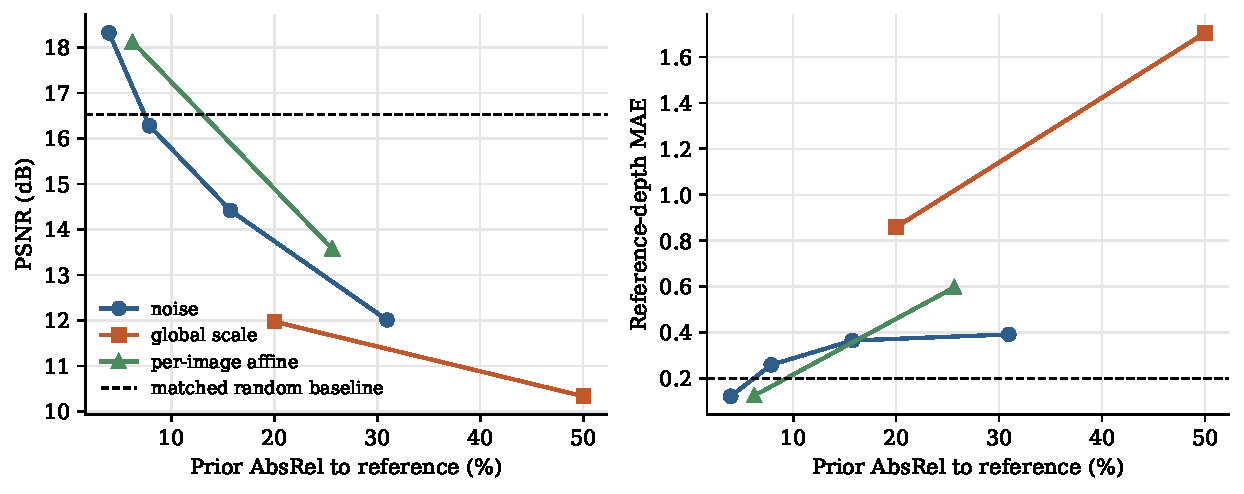
\includegraphics[width=0.92\linewidth]{report_corruption.pdf}
\caption{Matched corruption comparison from Table~\ref{tab:corruption}. Dashed lines
show the two-scene no-prior baseline. Curves connect sampled conditions and do not
estimate a continuous threshold. Equal horizontal positions would mean equal prior
AbsRel, not equivalent corruption structure.}
\label{fig:corruption}
\end{figure}

\paragraph{How the prior enters matters.} Figure~\ref{fig:paths} retains the broader
comparison of initialization only, loss only, and initialization plus loss for SSI and
absolute supervision. Errors introduced by backprojection remain consequential even
when the loss fits away affine disagreement. Loss-only SSI has a different
sensitivity, while absolute supervision directly exposes a miscalibrated target to
optimization. The distinction is visible in individual outcomes: a Lego
initialization-only per-image-affine prior at 6.2\% AbsRel raises PSNR by 0.72\,dB but
raises MAE by 51.8\%; a random-initialized SSI loss-only noise prior at 7.8\% AbsRel
lowers PSNR by 0.42\,dB while reducing MAE by 10.7\%. Thus similar prior-error
magnitudes do not determine either the direction of change or the mechanism of
failure.

\begin{figure}[!htbp]\centering
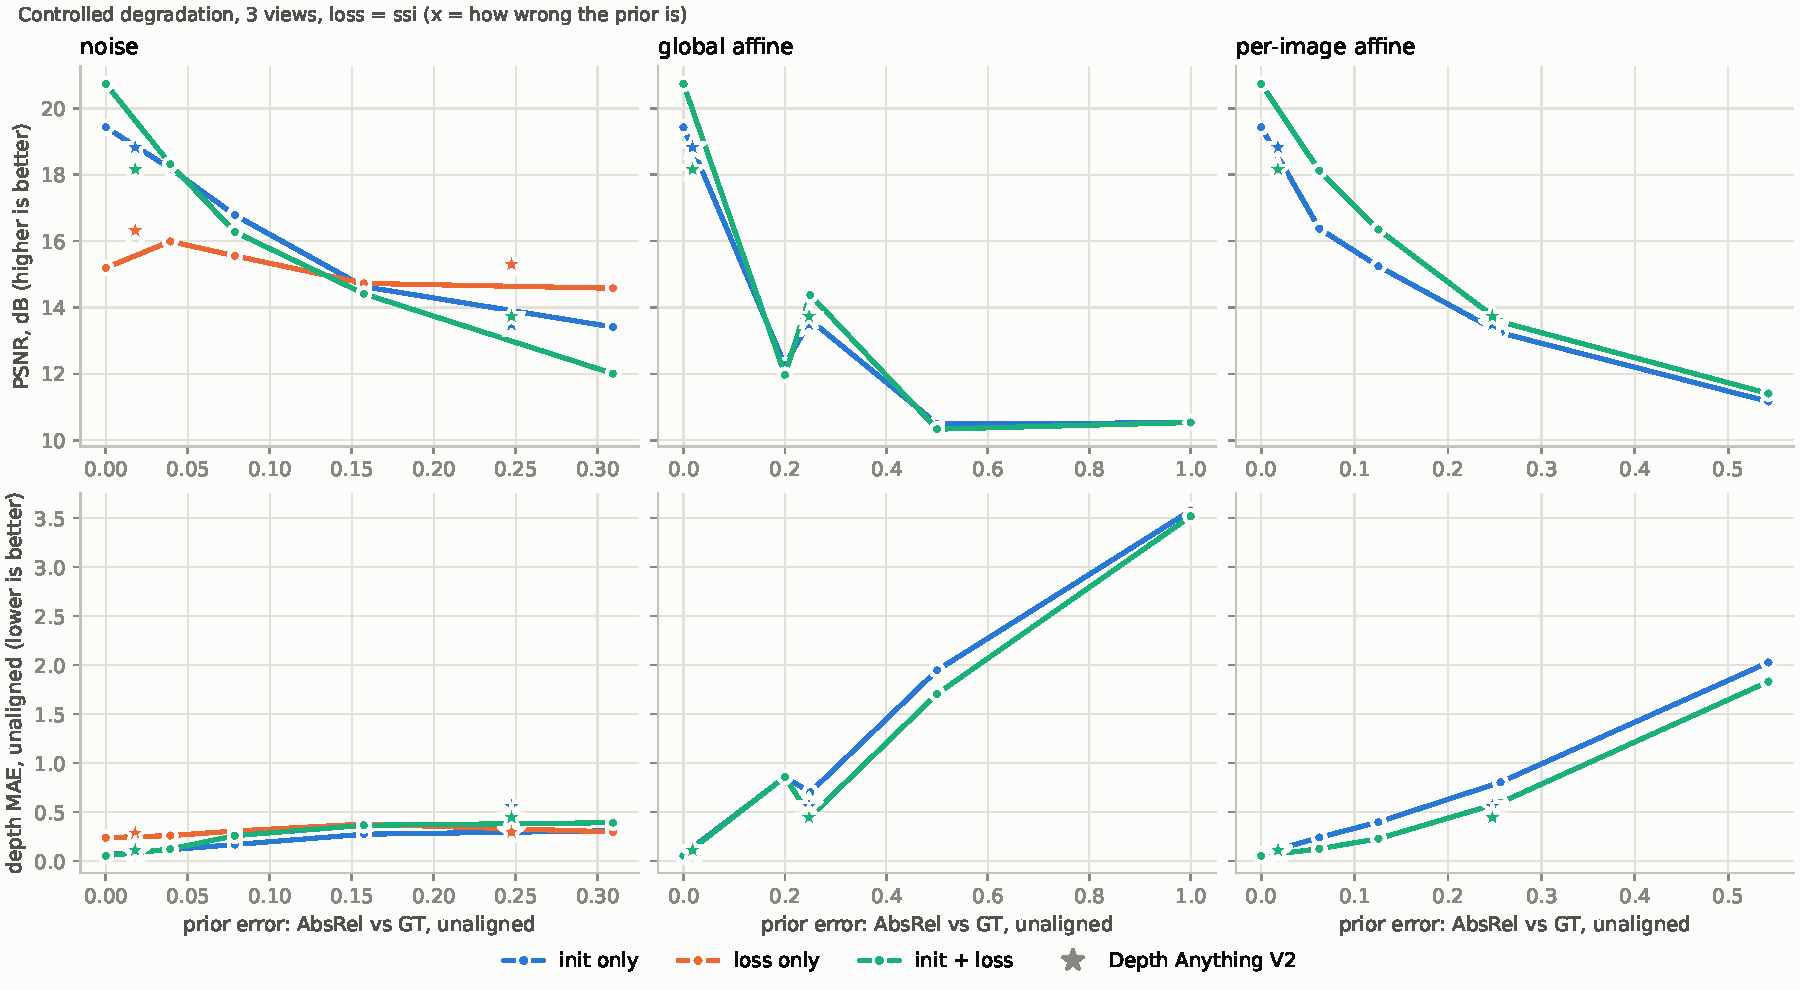
\includegraphics[width=0.74\linewidth]{degradation_ssi.pdf}\\[2pt]
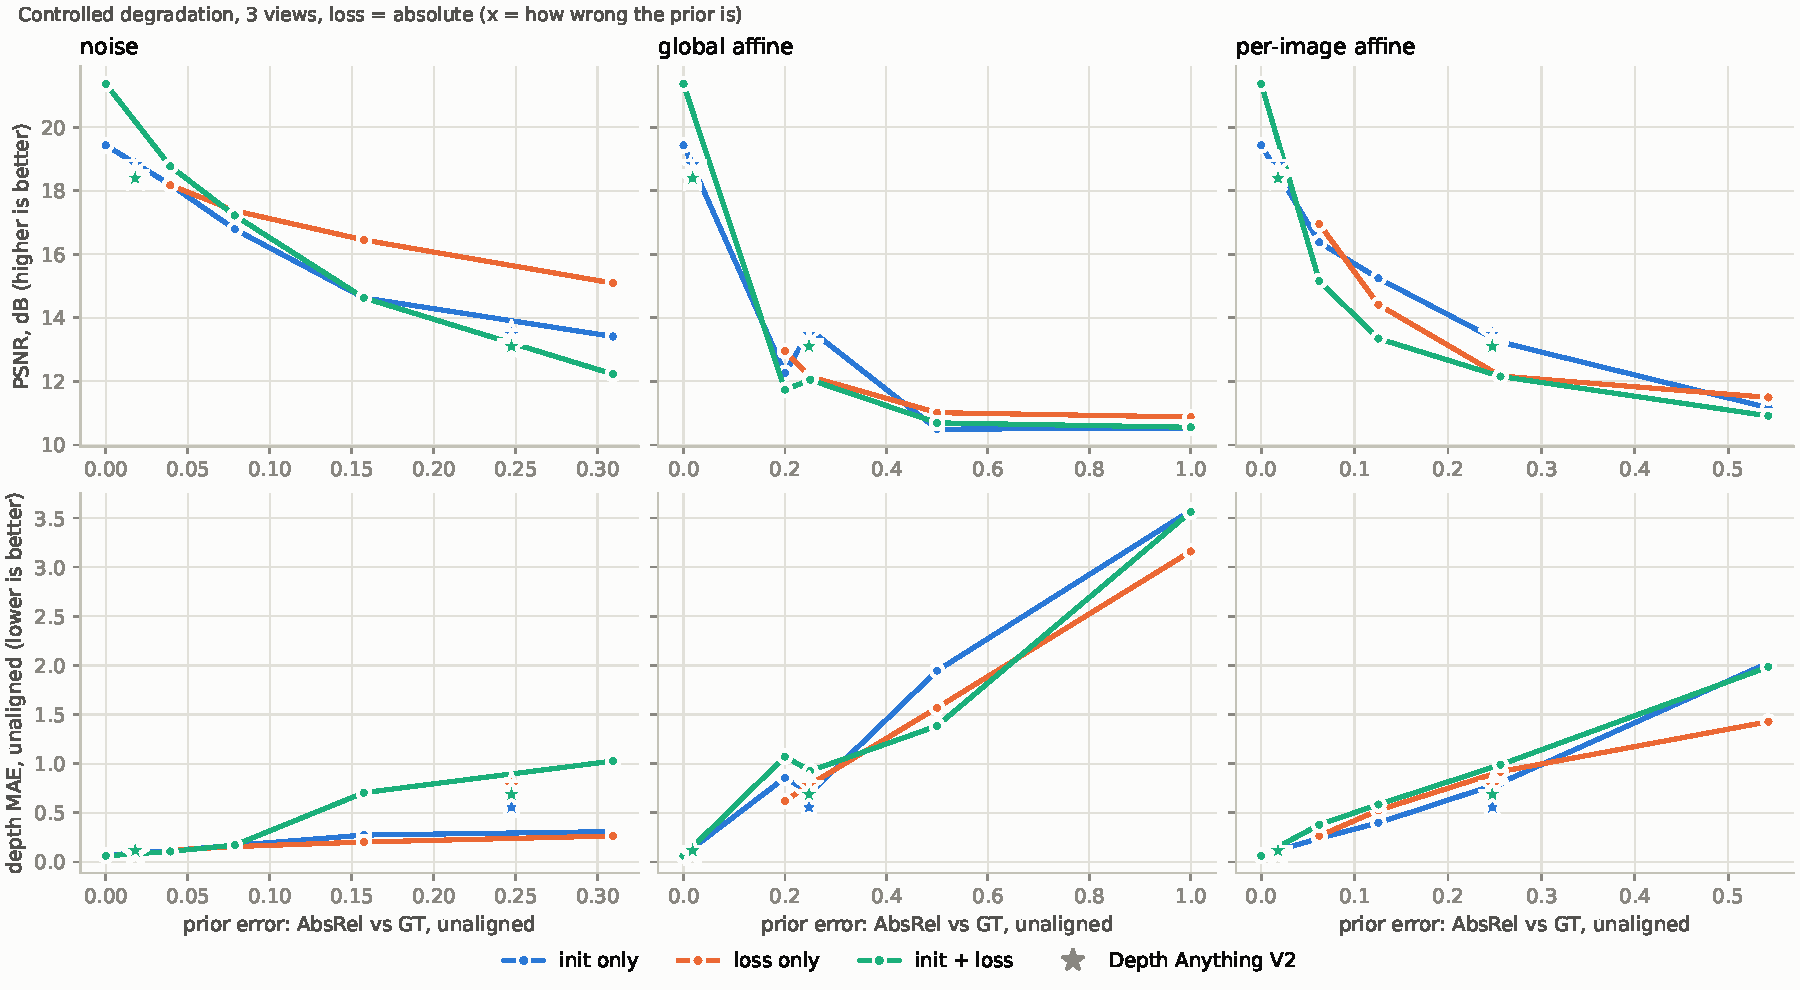
\includegraphics[width=0.74\linewidth]{degradation_absolute.pdf}
\caption{Three-view corruption curves across intervention paths: SSI supervision
(top) and absolute supervision (bottom). Each block plots PSNR above unaligned
reference-depth MAE, against prior AbsRel. Colors distinguish initialization only,
loss only, and initialization plus loss; stars show the real-model operating points.
Missing path/family combinations reflect the staged design and pruning, not measured
zero effect. Curves interpolate displayed configurations, without uncertainty bands.}
\label{fig:paths}
\end{figure}

\subsection{Depth Anything V2}

The controlled perturbations let us ask whether a real predictor operates in a useful
regime. We evaluate the large Depth Anything V2 model under reference-assisted oracle
calibration and sparse-SfM-assisted calibration (Section~3.1).
Table~\ref{tab:dav2} summarizes the synthetic three-view results. With
reference-assisted calibration, prior AbsRel is 1.8\%, and the depth-initialized
configurations reach 18.2--18.8\,dB PSNR with MAE 0.085--0.115. Under the tested
SfM-assisted pipeline, prior AbsRel is 24.7\%, with 13.1--13.7\,dB PSNR and MAE
0.44--0.69. The former is useful relative to the two-scene no-prior baseline; the
latter degrades both measurements.

An additional per-image affine diagnostic reduces the SfM-calibrated prior's residual
AbsRel to 3.5\%. This indicates a substantial affine component in the depth
disagreement, but does not establish which part of the calibration caused it. The
calibration is performed in inverse-depth space before inversion, and the SfM fit
uses 6--7 points per view on average. The small number of synthetic SfM
correspondences is a plausible contributor, but was not varied independently and
cannot by itself explain the entire difference.

\begin{table}[!htbp]\centering\small
\caption{Depth Anything V2 Large on the synthetic three-view setting. PSNR and MAE
intervals span the three depth-initialized configurations under each calibration
condition (initialization only, and with SSI or absolute loss at $\lambda=0.1$); they
are not confidence intervals. The loss-only configuration with random initialization
falls outside these intervals (16.3\,dB / 0.284 oracle; 15.3\,dB / 0.296 SfM-assisted).
Oracle calibration uses reference information unavailable in a normal sparse-view
reconstruction.}
\label{tab:dav2}
\begin{tabular}{lrrr}
\toprule
Calibration condition & Prior AbsRel & PSNR (dB) & Reference MAE\\
\midrule
Reference-assisted (oracle) & 1.8\% & 18.2--18.8 & 0.085--0.115\\
Three-view SfM-assisted & 24.7\% & 13.1--13.7 & 0.44--0.69\\
\bottomrule
\end{tabular}
\end{table}

Figure~\ref{fig:qualitative} illustrates the consequence on a held-out Lego view.
Clean-reference initialization gives more coherent RGB and rendered depth than the
random baseline. A scale-biased initialization disrupts both, and the tested
SfM-calibrated real-model configuration also produces a degraded reconstruction. The
depth panels visualize spatial structure; without a shared numerical color scale,
color differences should not be read as calibrated depth-error measurements.

\begin{figure}[!htbp]\centering
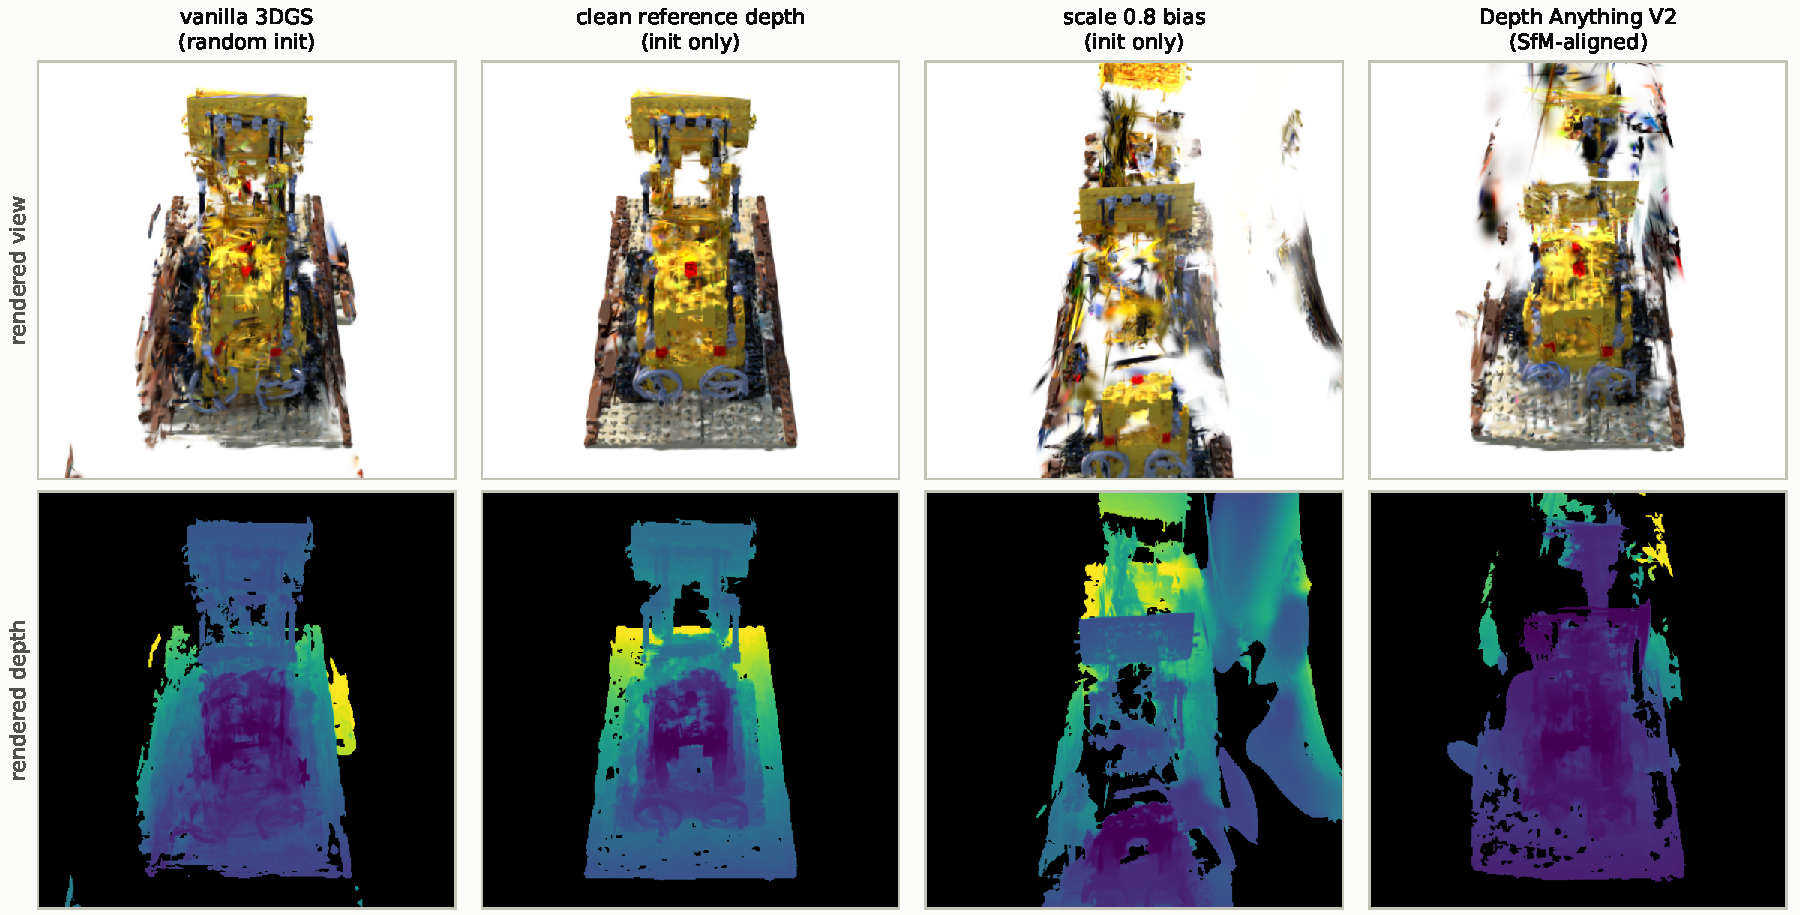
\includegraphics[width=\linewidth]{qualitative.pdf}
\caption{Qualitative three-view Lego comparison at the same held-out camera. These are
rendered RGB images and expected-depth maps, not ground-truth surface maps. The
comparison illustrates reconstruction behavior under clean, corrupted, and real-model
priors; quantitative conclusions use the corresponding evaluation metrics.}
\label{fig:qualitative}
\end{figure}

\subsection{DTU real-scene validation}

We next ask whether depth benefits extend to geometry measured independently of a
learned reconstruction. Table~\ref{tab:dtu} compares the tested pipelines on DTU
scans 1 and 6. At three views, Depth Anything V2 initialization reduces mean Chamfer
from the random baseline's 5.010\,mm to 2.750\,mm, a 45.1\% reduction, while PSNR
increases from 8.77 to 12.11\,dB. At nine views, the corresponding Chamfer scores are
5.247 and 1.786\,mm. The SfM-initialized pipeline with DAv2 depth loss achieves the
highest PSNR among the displayed pipelines, reaching 20.43\,dB at nine views, while
its 1.374\,mm Chamfer remains above the clean-reference initialization result of
0.987\,mm.

The SfM rows isolate the DAv2 loss for a fixed initialization. At three views, adding
it raises PSNR by 2.51\,dB, and SSIM and LPIPS also improve (0.428 to 0.513 and 0.509
to 0.444), while Chamfer error grows by 13.3\% (3.445 to 3.902\,mm). At nine views it
improves both PSNR ($+1.57$\,dB) and Chamfer ($-16.1\%$). The remaining rows compare
complete pipelines; they do not isolate initialization from regularization or prove
that correspondence count alone explains the contrast with synthetic scenes.

\begin{table}[!htbp]\centering\small
\caption{DTU pipeline comparison, means over scans 1 and 6. Entries are full-image
PSNR in dB / structured-light Chamfer in mm. The structured-light reference and DAv2
depth-initialization rows use initialization only ($\lambda=0$); the SfM + DAv2 row
adds the SSI depth loss at $\lambda=0.1$ to the SfM initialization of the row below
it.}
\label{tab:dtu}
\begin{tabular}{lcc}
\toprule
Pipeline & 3 views & 9 views\\
\midrule
Structured-light reference initialization & 11.73 / 1.218 & 17.33 / 0.987\\
DAv2 depth initialization & 12.11 / 2.750 & 15.99 / 1.786\\
SfM initialization + DAv2 depth loss & 13.47 / 3.901 & 20.43 / 1.374\\
SfM initialization, no depth & 10.96 / 3.445 & 18.86 / 1.639\\
Random initialization, no depth & 8.77 / 5.010 & 9.70 / 5.247\\
\bottomrule
\end{tabular}
\end{table}

\paragraph{A matched reference-depth loss ablation.} To isolate continued depth
supervision, we keep structured-light reference initialization fixed and compare
$\lambda=0$ with SSI at $\lambda=0.1$. Table~\ref{tab:dtuablation} reports all three
appearance metrics alongside Chamfer. At three views, mean Chamfer decreases from
1.2184 to 0.8042\,mm, a 34.0\% reduction, while PSNR decreases from 11.73 to
11.37\,dB. However, SSIM increases from 0.5999 to 0.6147 and LPIPS decreases from
0.3538 to 0.3411. Thus geometry improves while PSNR worsens, but both other appearance
metrics improve. Calling this simply a loss of appearance quality would obscure the
actual result.

At nine views, mean Chamfer decreases from 0.9867 to 0.6587\,mm, a 33.2\% reduction.
Mean PSNR and SSIM decrease, and LPIPS increases slightly. Both scans improve
geometrically at both view counts (Figure~\ref{fig:dtuscans}), but nine-view PSNR is
heterogeneous: it increases by 0.30\,dB on scan 1 and decreases by 1.19\,dB on
scan 6. These paired observations support a real geometry benefit while showing why
two-scan averages should not be treated as universal behavior.

\begin{table}[!htbp]\centering\small
\caption{Matched DTU reference-depth loss ablation, means over scans 1 and 6, with
identical reference initialization. The three-view loss improves Chamfer, SSIM, and
LPIPS despite reducing PSNR. Chamfer means are computed from the per-run
accuracy/completeness evaluation.}
\label{tab:dtuablation}
\begin{tabular}{ccrrrr}
\toprule
Views & SSI $\lambda$ & PSNR $\uparrow$ & SSIM $\uparrow$ & LPIPS $\downarrow$ & Chamfer (mm) $\downarrow$\\
\midrule
3 & 0 & 11.73 & 0.5999 & 0.3538 & 1.2184\\
3 & 0.1 & 11.37 & 0.6147 & 0.3411 & 0.8042\\
9 & 0 & 17.33 & 0.8127 & 0.2093 & 0.9867\\
9 & 0.1 & 16.88 & 0.8109 & 0.2128 & 0.6587\\
\bottomrule
\end{tabular}
\end{table}

\begin{figure}[!htbp]\centering
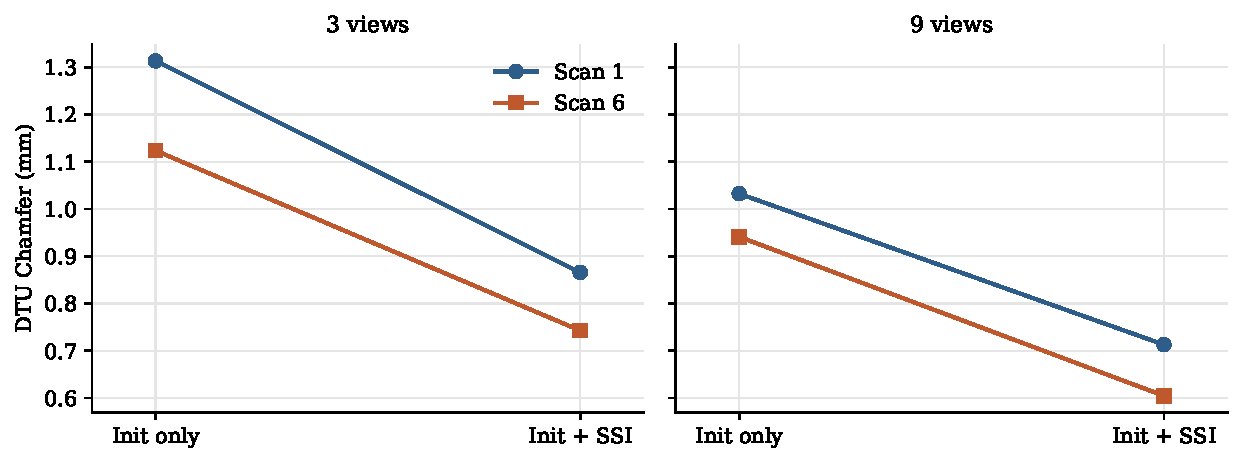
\includegraphics[width=0.92\linewidth]{report_dtu_scans.pdf}
\caption{DTU geometry improves on both scans when SSI supervision is added to
reference-depth initialization. Lines connect matched configurations for the same
scan; they are not error bars or repeated-seed confidence intervals.}
\label{fig:dtuscans}
\end{figure}

\subsection{Appearance--geometry divergence}

The preceding experiments distinguish two outcomes: joint degradation under a bad
prior, and opposing changes in image and geometric measurements.
Table~\ref{tab:divergence} gives five explicit depth-prior cases of the latter
relative to matched random baselines. Three have higher PSNR but worse reference-depth
MAE; two have lower PSNR but better MAE. The per-image-affine initialization-only Lego
case is particularly clear: PSNR increases by 0.72\,dB while MAE increases by 51.8\%.
The three per-image-affine cases change MAE by 0.048--0.087 in absolute terms, beyond
the largest shift the reference's own error could cause; the two noise cases ($-0.015$
and $-0.023$) are not (Section~\ref{sec:refcheck}). The DTU result above is unaffected
by the synthetic reference and gives a real-scene case: adding the DAv2 loss to SfM
initialization at three views improves all three appearance metrics while Chamfer
error grows by 13.3\%. The selected loss-weight comparisons and DTU ablation provide
additional examples under a different baseline definition.

\begin{table}[!htbp]\centering\small
\caption{Selected depth-prior divergences at three views. Each change is relative to
that scene's random-initialization, no-depth baseline. All rows use a depth prior
through initialization, a loss, or both. A positive MAE change means worse
reference-depth agreement.}
\label{tab:divergence}
\begin{tabular}{lllcrr}
\toprule
Scene & Prior & Path & Loss / $\lambda$ & $\Delta$PSNR & $\Delta$MAE\\
\midrule
Lego & Per-image affine & Init only & --- / 0 & $+0.72$ & $+51.8\%$\\
Lego & Per-image affine & Loss only & Absolute / 0.1 & $+0.69$ & $+34.1\%$\\
Lego & Noise & Loss only & SSI / 0.1 & $-0.42$ & $-10.7\%$\\
Chair & Noise & Init only & --- / 0 & $-0.41$ & $-8.9\%$\\
Chair & Per-image affine & Loss only & Absolute / 0.1 & $+0.17$ & $+33.9\%$\\
\bottomrule
\end{tabular}
\end{table}

Figure~\ref{fig:tradeoff} summarizes the broader configuration outcomes. Large joint
degradations occupy the upper-left region, while the upper-right region shows higher
PSNR with greater geometric error. The plot illustrates the diversity and scale of
responses across the study. Neither these selected examples nor the staged grid
provides an unbiased estimate of how frequently divergence occurs. In addition, PSNR
divergence should not be interpreted as disagreement with all appearance metrics, as
the three-view DTU results demonstrate.

\begin{figure}[!htbp]\centering
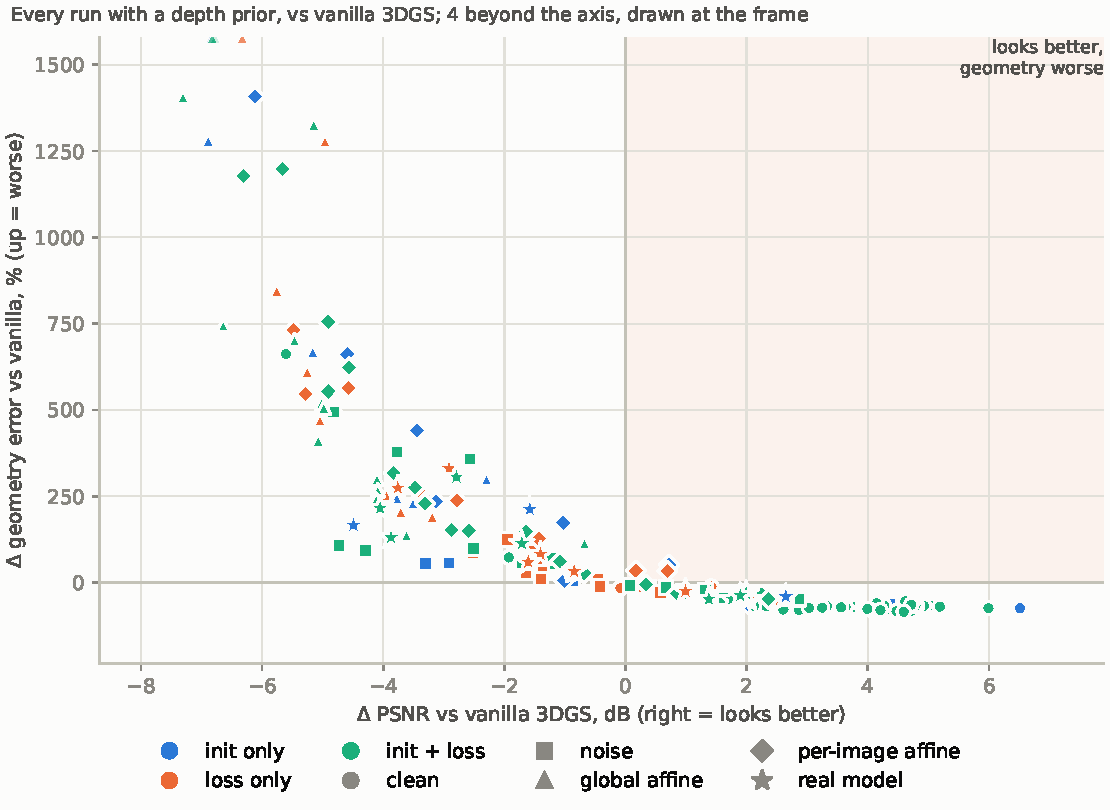
\includegraphics[width=0.8\linewidth]{tradeoff_map.pdf}
\caption{Broad appearance--geometry summary for depth-prior configurations. Horizontal
position is PSNR change from the matched no-prior baseline; vertical position is
relative geometry-error change (reference-depth MAE on synthetic scenes and Chamfer on
DTU). Colors indicate intervention paths and shapes prior families. Four out-of-range
points are drawn at the frame, so their boundary positions are clipped. The shaded
upper-right region represents higher PSNR with worse geometry. The plot supports
qualitative comparison of outcomes, not a divergence-frequency estimate or a common
absolute geometry scale.}
\label{fig:tradeoff}
\end{figure}

\subsection{What the reference error can change}\label{sec:refcheck}

Appearance metrics and DTU Chamfer do not use the dense reference. For synthetic
geometry, a run's MAE against the reference differs from its MAE against exact depth
by at most the reference's own MAE at the evaluation views, which is 0.008 on Lego,
0.013 on Chair, and 0.093 on Ship; a difference between two runs can therefore shift
by at most twice that. The corruption thresholds, the loss-family comparisons, and the
Depth Anything V2 operating points rest on Lego and Chair, where the smallest
corruption swept (3.9\%) is 10--18 times the reference's AbsRel and the
oracle-calibrated Depth Anything V2 prior (1.8\%) 5--8 times. Ship enters only the
initialization and view-count comparisons: its clean-reference prior is effectively a
2.4\%-error prior on the input views, and excluding it leaves the advantage of clean-reference
initialization intact (Section~\ref{sec:init}). Under the worst-case bound, the
per-image-affine divergences of Table~\ref{tab:divergence} stand, whereas the four
clean-prior steps of Table~\ref{tab:lossablation} and the two noise divergences of
Table~\ref{tab:divergence} are too small to rule out reference error.

\section{Discussion}

The study identifies three distinct decisions behind a successful depth intervention.
The first is whether the prior supplies useful initial geometry. Clean-reference
initialization is consistently strong in the controlled synthetic experiment, but a
coherent scale error can place the starting points so poorly that RGB optimization
does not repair them. An invariant loss cannot undo this initialization error merely
by ignoring affine disagreement.

The second decision is how strongly to constrain the subsequent optimization. The
loss sweep and matched ablations show that more depth supervision is not uniformly
better, even with clean depth. SSI, Pearson, and absolute losses impose different
constraints, and their numerical weights are not interchangeable. Loss selection
should therefore account for calibration quality, view coverage, and the metric
relevant to the application.

The third decision concerns what counts as improvement. Synthetic MAE measures
agreement with a dense learned reference, which exact Blender depth shows to be
accurate on Lego and Chair but not on Ship's water; DTU Chamfer measures agreement
with independently acquired geometry. PSNR, SSIM, and LPIPS also capture different
aspects of rendering quality. On DTU at three views, reference-depth supervision
improves geometry, structure, and perceptual similarity together while PSNR declines,
and a DAv2 loss improves all three appearance metrics while geometry worsens. A single
scalar conceals both distinctions.

Practically, we recommend validating prior calibration and cross-view consistency
before backprojection, comparing initialization-only and loss-based interventions
against matched baselines, and inspecting geometry together with several appearance
metrics. The tested noise transition and moderate SSI weight are useful operating
observations, not deployment guarantees. The real-model results reinforce this point:
the same predictor can be useful or harmful under different calibration and scene
conditions.

\section{Limitations}

The main controlled study covers only three NeRF-Synthetic scenes, with the corruption
experiments concentrated on Lego and Chair, and real-scene validation covers only two
DTU scans. The synthetic reference is a dense learned reconstruction rather than exact
depth; measured against exact Blender depth, it is accurate to 0.4\% on Lego and Chair
but 2.3\% off on Ship, which limits how finely Ship's geometry numbers can be read.
Clean-reference experiments deliberately use oracle information, including dense-view
information beyond the sparse training set. Every configuration was trained once, with
a single seed, and the staged sweep does not sample all configurations uniformly, so
small differences and event frequencies should not be generalized. The real-model
comparison does not independently isolate calibration domain, correspondence count,
and scene content. Finally, SH degree zero in the main study and full-image DTU
appearance evaluation restrict comparisons with other reconstruction settings.

\section{Conclusion}

Depth priors can substantially improve sparse-view 3DGS, but their value depends on
initialization, supervision, view coverage, and calibration. Clean dense-reference
initialization improves both PSNR and reference-depth agreement, whereas corrupted
priors can erase or reverse these gains. Coherent affine errors are especially
damaging in the tested configurations, and selected experiments demonstrate that PSNR
and geometry can move in opposite directions. Depth Anything V2 provides a useful
empirical test of these issues, while DTU confirms that depth information can improve
independently measured real-scene geometry. A reliable evaluation should therefore
report calibration-sensitive geometry and multiple appearance metrics, with
conclusions tied to matched experimental conditions rather than a universal threshold
or loss weight.

\begin{thebibliography}{99}\small
\bibitem{kerbl2023} B.~Kerbl, G.~Kopanas, T.~Leimk\"uhler, and G.~Drettakis. 3D
Gaussian Splatting for Real-Time Radiance Field Rendering. \emph{ACM Transactions on
Graphics}, 42(4), 2023.
\bibitem{foroutan2024} Y.~Foroutan, D.~Rebain, K.~M.~Yi, and A.~Tagliasacchi.
Evaluating Alternatives to SFM Point Cloud Initialization for Gaussian Splatting.
arXiv:2404.12547, 2024.
\bibitem{li2024} J.~Li, J.~Zhang, X.~Bai, J.~Zheng, X.~Ning, J.~Zhou, and L.~Gu.
DNGaussian: Optimizing Sparse-View 3D Gaussian Radiance Fields with Global-Local Depth
Normalization. \emph{CVPR}, 2024.
\bibitem{yang2024} L.~Yang, B.~Kang, Z.~Huang, Z.~Zhao, X.~Xu, J.~Feng, and H.~Zhao.
Depth Anything V2. \emph{NeurIPS}, 2024.
\bibitem{mildenhall2020} B.~Mildenhall, P.~P.~Srinivasan, M.~Tancik, J.~T.~Barron,
R.~Ramamoorthi, and R.~Ng. NeRF: Representing Scenes as Neural Radiance Fields for
View Synthesis. \emph{ECCV}, 2020.
\bibitem{jensen2014} R.~Jensen, A.~Dahl, G.~Vogiatzis, E.~Tola, and H.~Aan\ae s. Large
Scale Multi-view Stereopsis Evaluation. \emph{CVPR}, 2014.
\bibitem{ye2025} V.~Ye, R.~Li, J.~Kerr, M.~Turkulainen, B.~Yi, Z.~Pan, O.~Seiskari,
J.~Ye, J.~Hu, M.~Tancik, and A.~Kanazawa. gsplat: An Open-Source Library for Gaussian
Splatting. \emph{Journal of Machine Learning Research}, 26(34):1--17, 2025.
\end{thebibliography}

\end{document}
